\documentclass{beamer}
\usetheme{Boadilla}
\usecolortheme{sidebartab}

\usepackage{hyperref}
\usepackage{showexpl} 
\usepackage{graphicx}
\usepackage{color}
\usepackage{siunitx}
\usepackage[version=3]{mhchem}
\usepackage{chemfig}
\usepackage{changes}
\usepackage[many]{tcolorbox}
\usepackage{natbib}
\bibliographystyle{unsrtnat}
\setcitestyle{square,numbers}

\beamertemplatenavigationsymbolsempty
\setbeamertemplate{footline}{}
\setbeamertemplate{bibliography item}{\insertbiblabel}

\lstloadlanguages{[LaTeX]Tex} 
\lstset{% 
     basicstyle=\ttfamily\large, 
     commentstyle=\itshape\ttfamily, 
     showspaces=false, 
     showstringspaces=false, 
     breaklines=true, 
     breakautoindent=false, 
     captionpos=t,
     explpreset={numbers=none},
     pos=b
} 

\title{Sharing and Archiving Research Data}
\author{Markus Stocker}
\date{September 12, 2017}

\begin{document}

\maketitle

\begin{frame}
  \frametitle{Outline}
  
  \begin{itemize}
  \item Open Data imperative
  \item How to share data
  \item Data repositories
  \item Credit for publishing data
  \end{itemize}
\end{frame}

\begin{frame}
  \frametitle{Open Data}
  
  \begin{itemize}
  \item Research data are assets
  \item Increasingly recognized and valued research output	
  \item Valuable to others, in research as well as industry
  \item Critical for reproducibility
  \item Mandates to open access publicly funded data
  \item Anyone free to use, reuse, and redistribute
  \item Possibly subject to attribution
  \end{itemize}
\end{frame}

\begin{frame}
  \frametitle{Why Sharing Data}
  
  \begin{itemize}
  \item Get credit for your work
  \item Share it with \emph{your future self}
  \item Enable reproducibility and repurposing of your data
  \item Increase visibility of your work
  \item Access to data (and software) seen positively in peer-review
  \item Because you are required to do so
  \item Because ``research data is not mine''
  \end{itemize}
  \tiny
  \begin{flushright}
  \url{https://www.linkedin.com/pulse/repeat-me-research-data-mine-wainer-lusoli}
  \end{flushright}
\end{frame}

\begin{frame}
  \frametitle{How to Share Data}
  
  \begin{itemize}
  \item It is challenging to share data well
  \item Making data usable by others in other contexts is difficult
  \item Study and follow existing principles and guidelines
  \item Share your data using a high-quality repository
  \end{itemize}
\end{frame}

\begin{frame}
  \frametitle{FAIR Principles}
  
  \begin{itemize}
  \item Findable
  \begin{itemize}
  \item Persistently identified, described, indexed
  \end{itemize}
  \item Accessible
  \begin{itemize}
  \item Retrievable by identifier, open protocol, accessible metadata
  \end{itemize}
  \item Interoperable
  \begin{itemize}
  \item Represented using formal, accessible, shared FAIR vocabulary
  \end{itemize}
  \item Re-usable
  \begin{itemize}
  \item Meet community standards, associate with provenance, usage license
  \end{itemize}
  \end{itemize}
  \tiny
  \begin{flushright}
  \url{https://www.force11.org/group/fairgroup/fairprinciples}
  \end{flushright}
\end{frame}

\begin{frame}
  \frametitle{Five Star Data}
  
  \begin{tabular}{rl}
  * & Publish your data on the web, open license, any format \\
  ** & Publish your data as structured data \\
  *** & Publish your data in a non-proprietary open format\\
  **** & Use identifiers to refer to your data, e.g. units, parameters \\
  ***** & Link your data to other data, to provide context \\
  \end{tabular}
  \tiny
  \begin{flushright}
  \url{http://5stardata.info/en/}
  \end{flushright}
\end{frame}

\begin{frame}
  \frametitle{Data Identification}
  
  \begin{itemize}
  \item Persistent identification of data is important
  \item Idea is similar to identification of articles
  \item Provides an unambiguous reference to data
  \item Used to link or refer to data, e.g. in text
  \item Data are increasingly identified by DOI 
  \begin{itemize}
  \item e.g. 10.1594/PANGAEA.787617
  \end{itemize}
  \item DataCite is the global provider of DOIs for research data
  \end{itemize}
\end{frame}

\begin{frame}
  \frametitle{Data Citation}
  
  \begin{itemize}
  \item Always cite data used in research
  \item Citing data is often very easy
  \item Similar to citing literature
  \item Data repositories often support citation export
  \item Exports in standard formats, supported by tools
  \end{itemize}
\end{frame}

{
	\usebackgroundtemplate{ %
		\begin{tikzpicture}[remember picture, overlay]%
		\node at (current page.center) {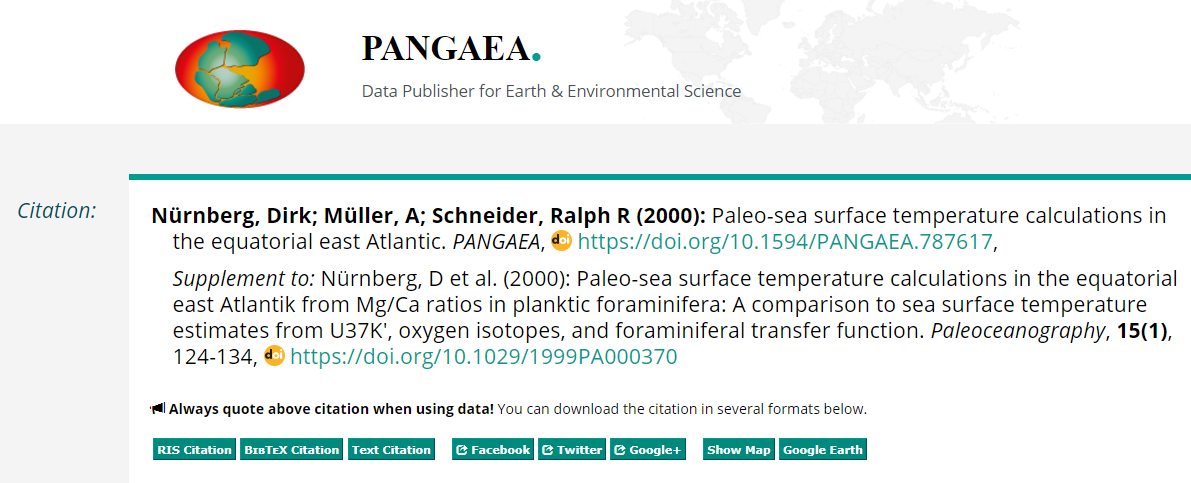
\includegraphics[width=\paperwidth]{graphics/pangaea-datacitation.png}};%
		\end{tikzpicture}%
	}%
	\setbeamertemplate{navigation symbols}{}
	\begin{frame}[plain]
	\end{frame}
}

\begin{frame}
  \frametitle{Data Repositories}
  
  \begin{itemize}
  \item re3data.org knows of 1920 research data repositories
  \item Covers major subjects and many special domains
  \item Quality varies widely
  \item Good quality data repository may meet many principles
  \item Support for data identification, citation, curation, standardization
  \item About 150 repositories are DSA or WDS certified
  \end{itemize}
\end{frame}

{
	\usebackgroundtemplate{ %
		\begin{tikzpicture}[remember picture, overlay]%
		\node at (current page.center) {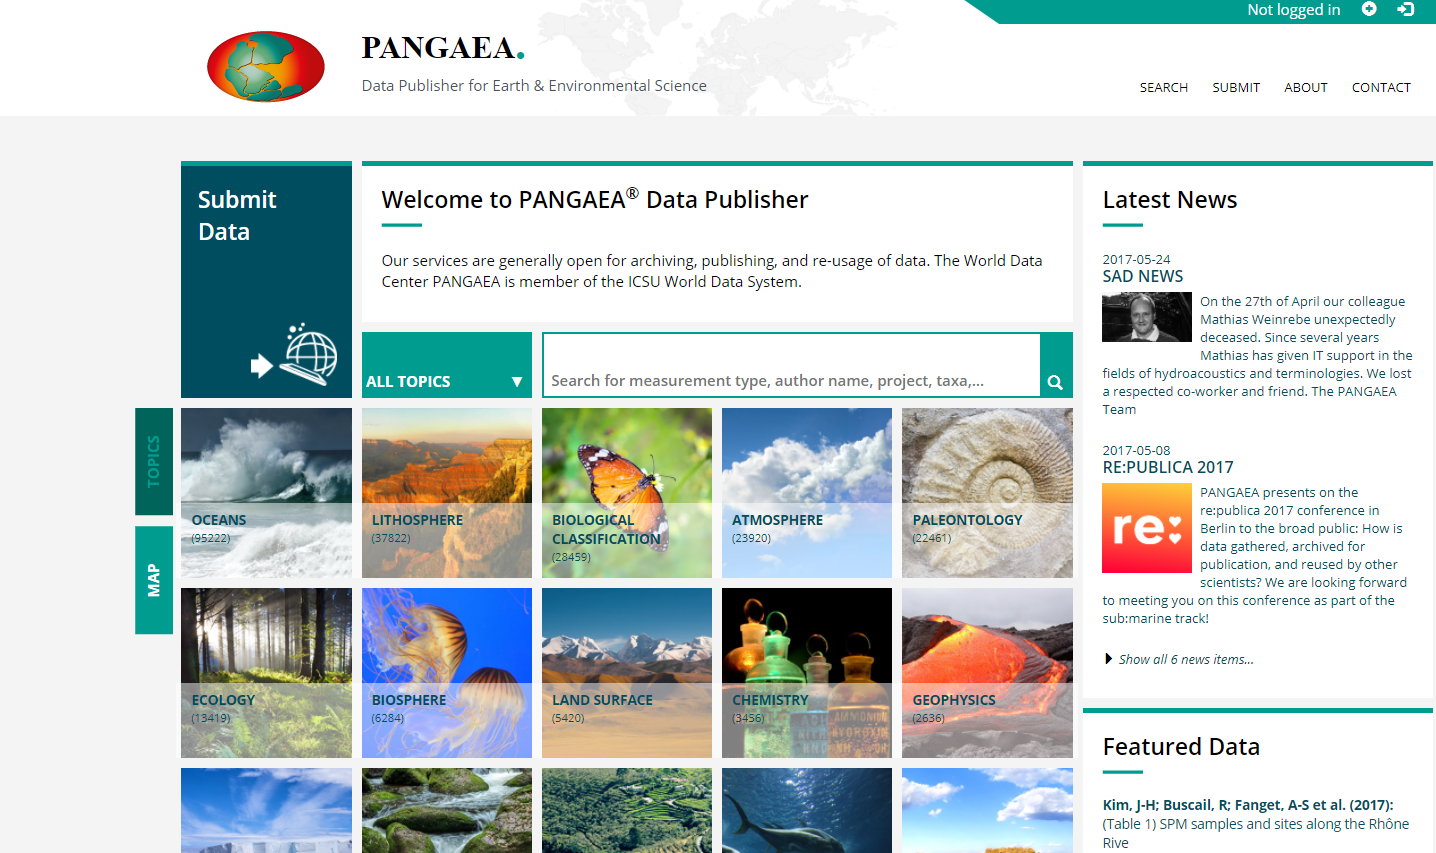
\includegraphics[width=\paperwidth]{graphics/pangaea.png}};%
		\end{tikzpicture}%
	}%
	\setbeamertemplate{navigation symbols}{}
	\begin{frame}[plain]
	\end{frame}
}

\begin{frame}
  \frametitle{PANGAEA}
  
  \begin{itemize}
  \item Open-access data publisher for earth and environmental science
  \item Archives, publishes, and distributes geo-referenced research data
  \item Can be used by any researcher to use, archive, publish data
  \item Published data are freely available
  \item Data and metadata canonicalized in relational database
  \item Data published in standard formats, accessed with standard protocols
  \item Data are identified and citable, using DataCite DOIs
  \item Data retrieval supported by full-text faceted search
  \item Cross-linking between data and articles
  \item Access to data warehouse
  \item Data undergo editorial process
  \item Ensures high usability of published data
  \end{itemize}
\end{frame}

\begin{frame}
  \frametitle{Other Repositories}
  
  \begin{itemize}
  \item re3data.org knows of 64 repositories in oceanography, e.g.
  \begin{itemize}
  \item Data Portal German Marine Research
  \item Marine Geoscience Data System
  \item World Data Service for Oceanography
  \end{itemize}
  \item Generic data repositories (not just data)
  \begin{itemize}
  \item figshare
  \item zenodo
  \item ResearchGate
  \end{itemize}
  \end{itemize}
\end{frame}

\begin{frame}
  \frametitle{Credit}
  
  \begin{itemize}
  \item Perhaps primary motivation to publish data
  \item Credit not as ``advanced'' as for articles, no d-index
  \item Article about the data used as workaround
  \item Demanded co-authorship on articles that use data
  \item Claim contributions to your ORCID record
  \end{itemize}
\end{frame}

\begin{frame}
  \frametitle{Take aways}
  
\end{frame}

\end{document}
